\chapter{Tugboats: Description and Operation}

A tug, or more commonly a tugboat, is an assistance boat which helps in the mooring or berthing operation of a ship by either towing or pushing a vessel towards the port \cite{SAAM} \cite{MarineInsight}.

Tugboats are also essential for non-self-propelled barges, oil platforms, log rafts, etc. Due to their solid structural engineering, tugs are small but relatively powerful machines.\\

This chapter presents the technical and operational characteristics of tugboats, with the aim of identifying design aspects for the hybrid propulsion system and the sizing of the battery bank.
% Breve descripción de qué se abordará y por qué es relevante.

\section{Overview of tugboats}
% Definir el tipo de embarcación con la que se está trabajando. Contextualizar qué tipo exacto de remolcador se está modelando

\begin{figure}[H]
    \begin{subfigure}{0.5\textwidth}
    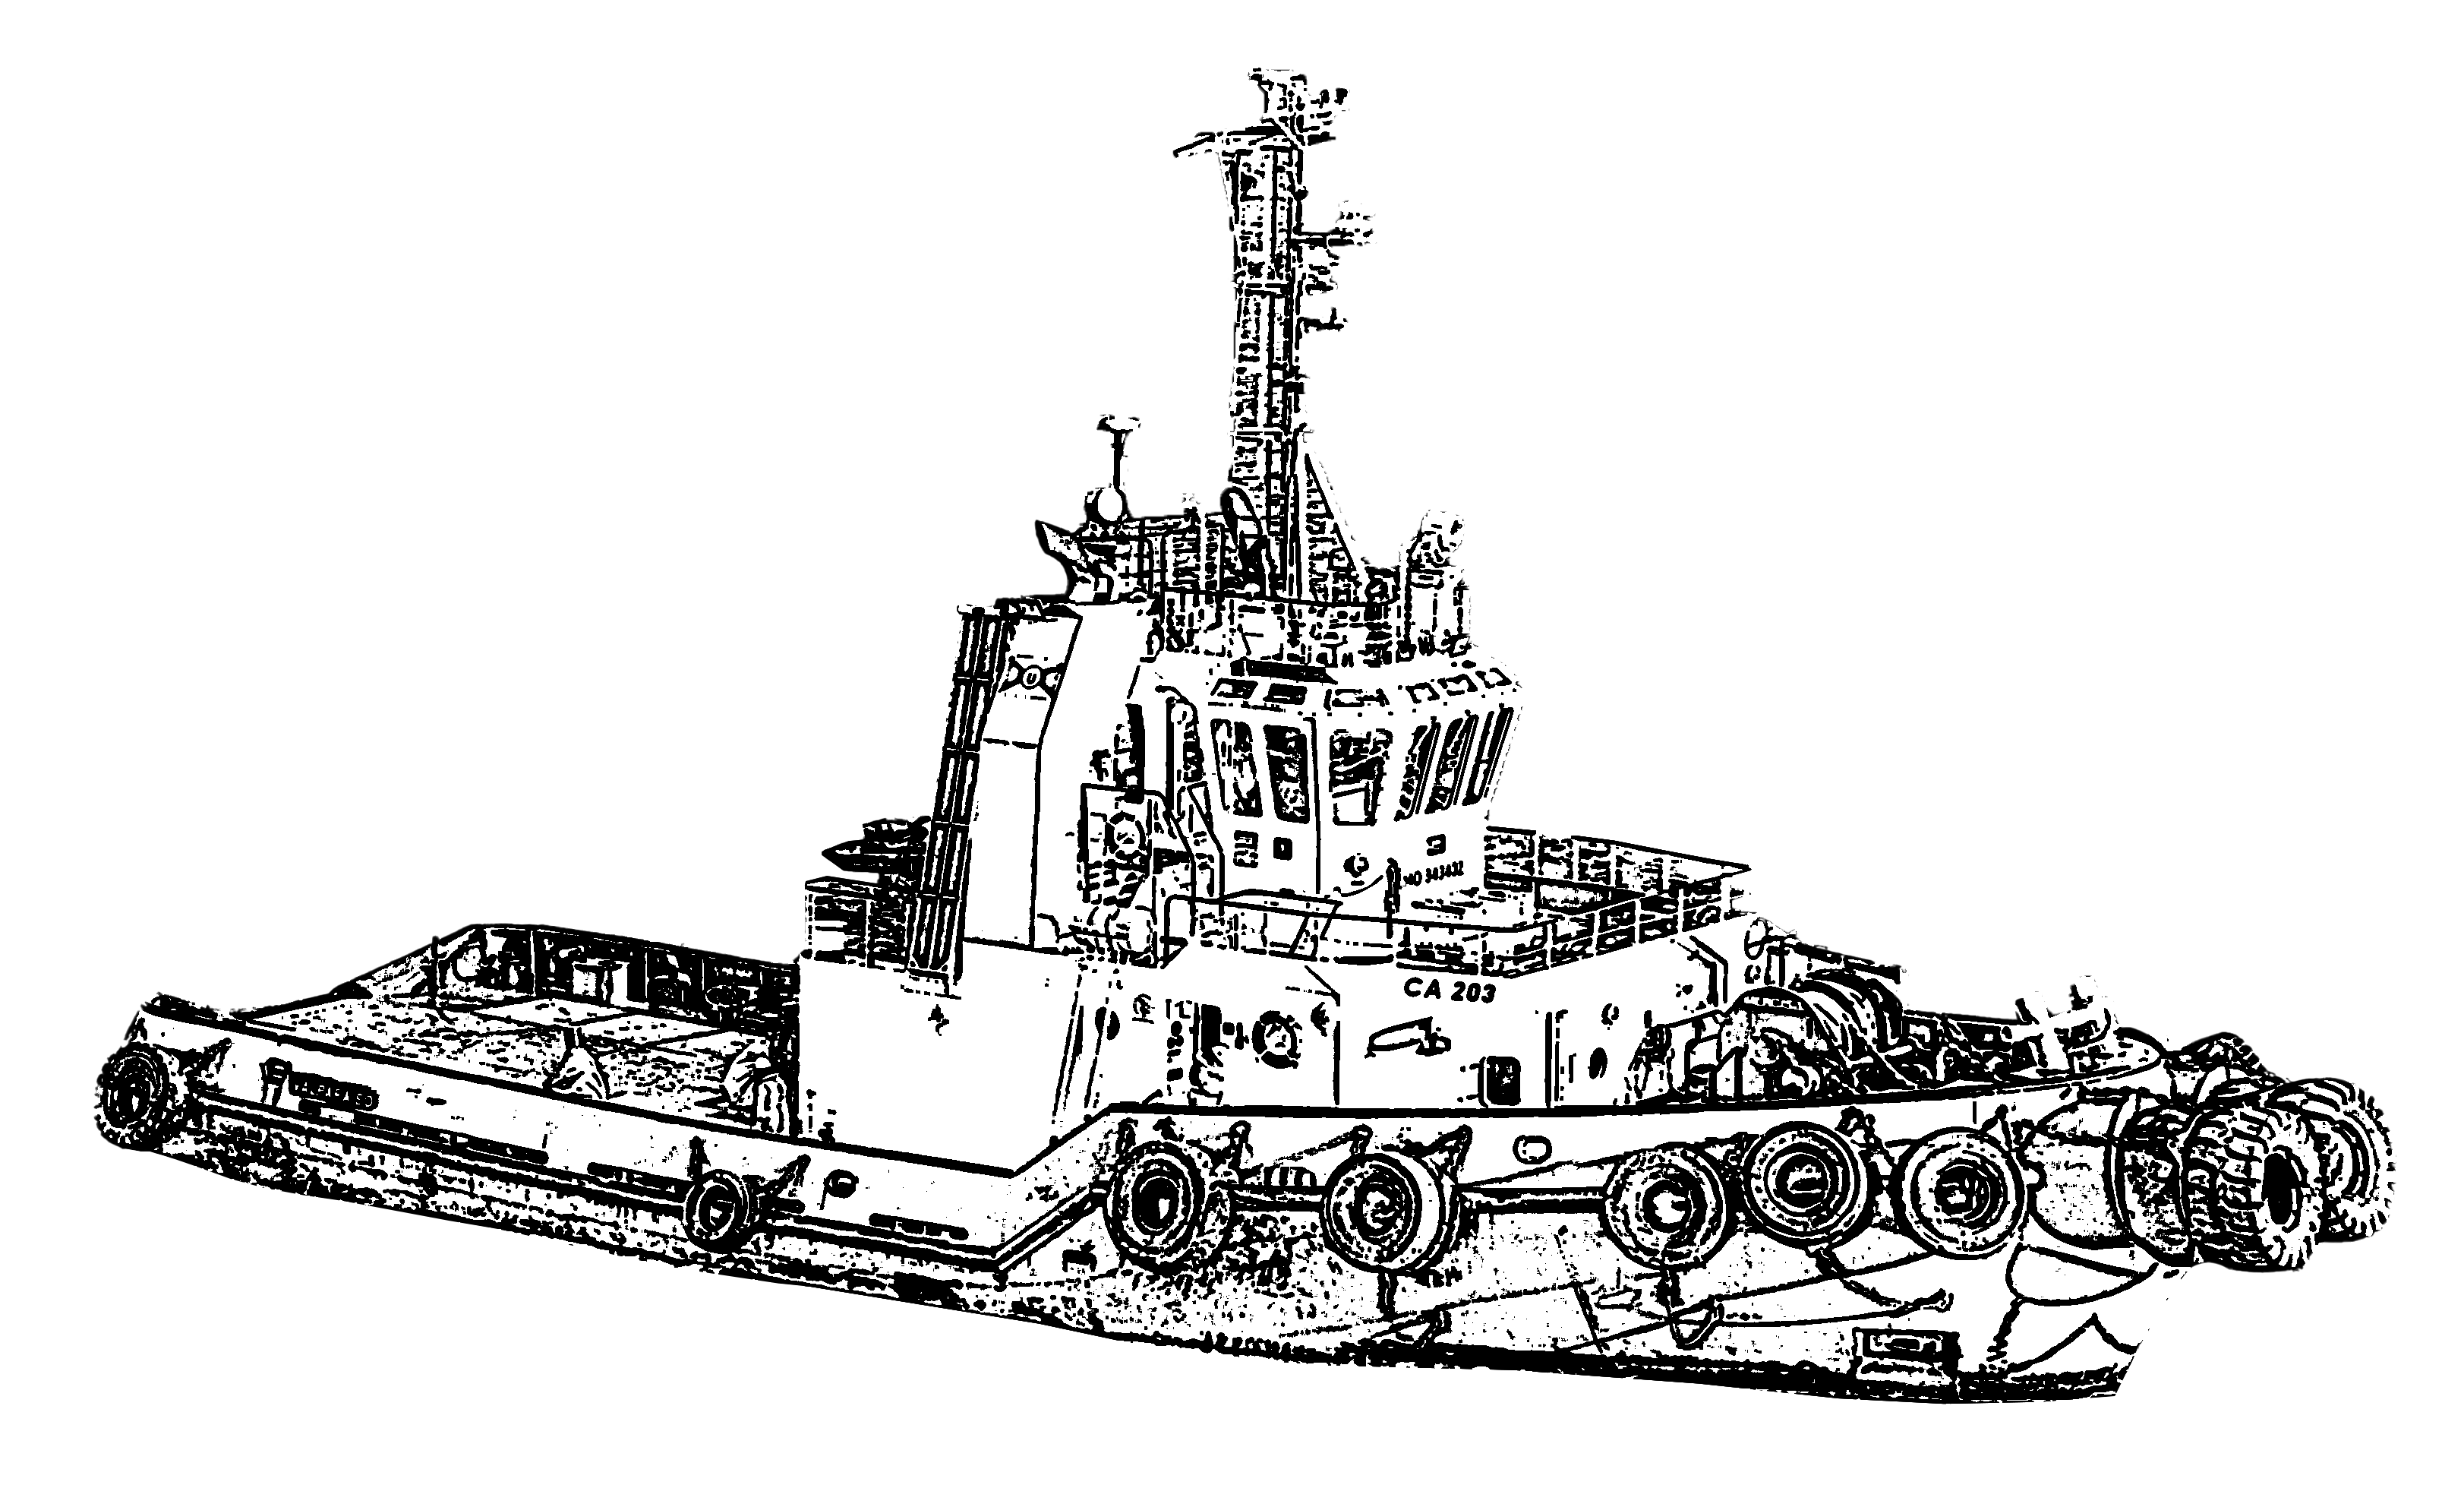
\includegraphics[width=1\textwidth]{images/chapter02/Remolcador.png}
    \caption{Conventional tug representation.}
    \label{fig:Tug1}
    \end{subfigure}
    \begin{subfigure}{0.5\textwidth}
    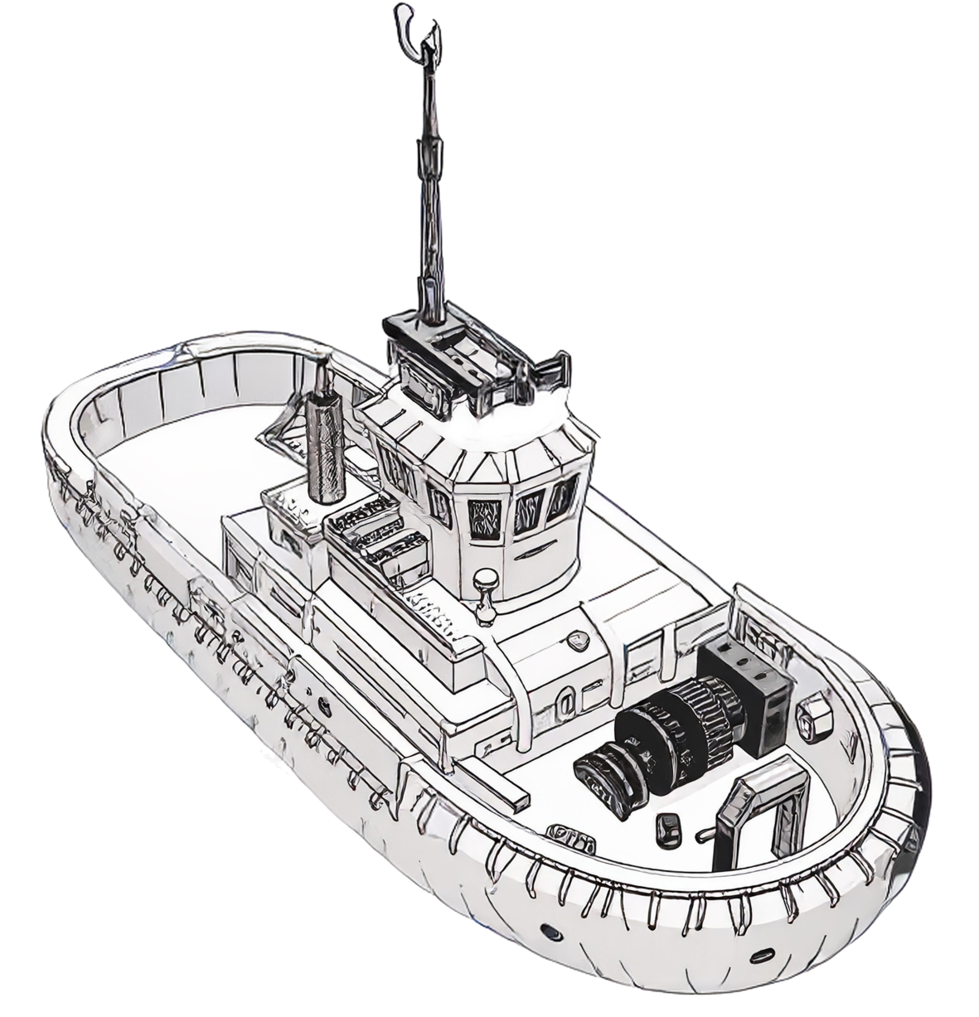
\includegraphics[width=0.7\textwidth]{images/chapter02/Remolcador2.png}
    \caption{Azimuth Tug representation}
    \label{fig:Tug2}
    \end{subfigure}    
    \caption{Tugs representations}
    \label{fig:Tugs}
\end{figure}

A tugboat is technically defined as a type of vessel specifically designed to assist other ships in moving by providing a controlled amount of force. They are essential vessels in ports, as is shown in fig. \ref{fig:Tugs}, where they assist in the movement of floating objects and in emergency tasks \cite{INEAL}.

In maritime law, maritime towing is defined as the operation whereby a vessel (the tugboat) transports another vessel or floating device that lacks self-propulsion or, despite having it, is unable to navigate under its own power, by pulling it through the sea. This functional duality—which encompasses both high-precision maneuvering assistance in congested environments (port towing) and long-distance transport and salvage (offshore towing)—requires design engineering and system redundancy adapted to very different operational risks \cite{Bruce}.

The importance of tugboats has grown exponentially with the phenomenon of naval gigantism \cite{Murimar}. Large modern ships, such as cruise ships and oil tankers, have tremendous momentum (inertia) that prevents them from stopping quickly or maneuvering effectively on their own in narrow channels or docks \cite{ESC_Group}.   

Therefore, tugboats are essential to counteract these inertial forces. Support is necessary for entry, exit, and general maneuvering, including assisting ships in emergency situations  \cite{Bruce}.   

Technological innovation plays a key role in tugboat operations. Environmental challenges and high efficiency requirements have driven the digitization and development of more sustainable and less polluting tugboats \cite{Murimar}. This trend includes the integration of automatic control technologies to optimize maneuver management, such as investment in hybrid and electric propulsion systems.\\\\     









The efficiency of these types of vessels is based on fuel consumption in relation to load capacities, always taking into account both the propulsion system and the energy conversion system that determines it. The efficiency of conventional propulsion systems varies between 38$\%$ and 41$\%$ for a power range between 100 kW and 2,500 kW. For vessels with higher power ratings, efficiency increases to 48$\%$ \cite{Griffiths} \cite{Wik}.

\subsection{Types of tugboats}
%(port, deep-sea, coastal, escort, etc.)
The classification of tugboats is primarily based on their operational domain and assigned primary mission. The usage and functions of tugs vary from port to port, as different ports have different requirements and intakes. The common thing is pushing or towing mega boats or barges. Their usage depends on the following factors:

\begin{itemize}
\item Port traffic Volume,
\item Types of ships to be served by that tug,
\item Navigational obstacles to be catered to,
\item Conditions of environmental protection,
\item Local laws and
\item Domains to be carried by a tug.
\end{itemize}

\subsubsection{a) Harbour Tugs}
These vessels are specialized in assisting large ships entering and leaving port limits. Their design prioritizes agility and the ability to apply force in any direction with maximum efficiency \cite{INEAL}. 

\begin{itemize}
	\item \textbf{Design:} Typical dimensions vary in length between 20 and 30 meters, with drafts of 3.0 to 4.5 meters. Their empty displacement speed ranges from 5 to 13 knots (9.3 - 24 km/h). The power of these tugboats can vary considerably, generally between 400 - 3,000 hp (300 and 2200 kW)\cite{IngeMarino}.
	
	
	\item \textbf{Propulsion:} Their designs have reduced length and increased beam and depth in order to install greater propulsion power, variable pitch propellers, Kort-type rotating nozzles with fixed rudders or rudder flaps, or Tow-Master systems (fixed nozzles with five rudders, two at the bow and three at the stern) to achieve greater traction and maneuverability \cite{IngeMarino} \cite{PracticosPuerto}.
\end{itemize}

\subsubsection{b) Offshore/SAR Tugs}
Designed to operate in the open sea, these tugboats are characterized by their robustness, greater autonomy, and ability to withstand severe ocean conditions.

\begin{itemize}
	 \item \textbf{Design:} Typical dimensions vary in length between 25 and 40 meters, with drafts of 4.5 to 6 meters. Their empty displacement speed ranges from 5 to 13 knots (9.3 - 24 km/h). The power of these tugboats can vary considerably, generally between 1500 - 6,000 hp (1120 - 4470 kW)\cite{IngeMarino}.

	\item \textbf{Multifunctionality:} In addition to long-distance towing tasks, they are equipped for rescues and complementary firefighting and pollution control tasks \cite{SalvamentoMaritimo}. An example of a modern rescue vessel is 40 meters long, has 5,300 hp and a Bollard Pull of 60 tons \cite{Cotecmar}. These vessels are equipped to provide any type of assistance to deep-draft vessels \cite{SalvamentoMaritimo}. 
\end{itemize}

\subsubsection{c) Escort Tugs}
These tugboats perform a critical safety mission. Their main objective is to provide preventive escort to ships carrying hazardous materials (such as LNG or crude oil) in high-risk areas, standing ready to counteract any possible loss of control of the assisted vessel.

\begin{itemize}

	\item \textbf{Design:} Typical dimensions vary in length between 40 and 80 meters, with drafts of 5 to 6 meters. Their empty displacement speed ranges from 15 to 16 knots (9.3 - 24 km/h). The power of these tugboats can vary considerably, generally between 6,000 -20,000 hp (4470 - 14,900 kW)\cite{IngeMarino}.

	\item \textbf{Technology and Bollard Pull:} They require extremely robust and powerful designs to maintain control of a vessel moving at cruising speeds. An example of a modern escort tugboat (\textit{Robert Allan Rastar 3200 model}) features Rolls Royce azimuth thrusters and is designed to generate fixed-point traction exceeding 85 tons \cite{PortalPortuario}. They are equipped with constant tension maneuvering winches to maximize safety during operations. 
\end{itemize}


\subsubsection{d) Tugs Comparation}

Below, in the table \ref{tab:Tugs}, there is a summary of key operational and dimensional characteristics:

\begin{table}[H]
	\centering
	\caption{Operational Classification and Dimensional Parameters of the Tugboat}
	\label{tab:Tugs}
	\begin{tabular}{c|p{35mm}|p{35mm}|c}
		\hline      \textbf{Type of Tugboat} & \textbf{Operation}  & \textbf{Design objective} & \textbf{Typical BP} \\		
\hline \hline
		Harbour Tug    & Protected maritime and port areas such as bays or estuaries. & Maneuverability, Reduced Draft & 40-80\\ \hline
		Offshore/SAR Tugs  & Open Ocean & Autonomy, Stability, SAR Power & 60-200+\\ \hline
		Escort Tugs  & High-Risk Areas (LNG, Crude Oil) & Rollover Control, Side Pull Capacity & 60-120\\
		\hline \hline
	\end{tabular}
\end{table}



\section{Technical Characteristics of the Propulsion System}

% Explicar las características mecánicas y eléctricas que determinan cómo debe diseñarse el sistema híbrido.

\subsection{Bollard Pull - BP}
Bollard pull (BP) is the fundamental metric for quantifying a tugboat's pulling power.

BP measures the maximum force a vessel can exert while stationary in the water. It is the maritime equivalent of horsepower or torque in land vehicles. The measurement requires securing the vessel to a fixed bollard at the dock and using specialized load cells to calculate the tension generated on the line with the engines running at full power.   

BP specifications are expressed in units such as kilonewtons (kN), short tons (stf), or ton-force (tf) and are critical for demonstrating the vessel's pulling capacity under load. All commercial vessels intended for towing operations must obtain fixed point pulling certification from international classification societies such as the American Bureau of Shipping (ABS) or Bureau Veritas (BV)\cite{Murimar}.   

The tugboat's design is specifically geared toward maximizing pulling force in relation to its size. A common and effective way to increase pulling force is by adding a nozzle (duct) that surrounds the propeller, which improves propulsive efficiency \cite{Murimar}. 

\subsection{Propulsion Engineering for Maneuvering}
The maneuverability of a tugboat, which directly influences its operational efficiency and safety, is intrinsically linked to the design of its propulsion system.

\subsubsection{a) Conventional Propulsion} It uses a standard diesel engine connected to a propeller. It is a proven and simple system, with good efficiency in linear towing tasks within ports and coastal areas. However, it offers limited lateral maneuverability compared to more advanced systems \cite{MJimenez}.

\subsubsection{b) ASD - Azimuthal Stern Drive} These are rotary thrusters, where a motor is capable of directing all its thrust in any direction \cite{MJimenez}. They all have two propellers, and since each one can be oriented independently, maneuverability is greatly increased, allowing them to turn on themselves in a single length \cite{JFarina}. The only difference with conventional tugboats are the modifications to the stern and structure to house the propellers and withstand the forces exerted by the nozzle rudder, which are different from those exerted by a conventional rudder and propeller \cite{JFarina}. 

\subsubsection{c) Voith-Schneider Propulsion (VSP)} This system offers omnidirectional thrust and total steering control, resulting in formidable positioning accuracy. These harbor tugs have been equipped with \textit{VoithSchneider} propellers, a unique type of propulsion system consisting of oscillating blades that allow them to have total, targeted control over the vessel without having to adjust the orientation of the main engine or propellers \cite{MJimenez}.

This propulsion system allows for highly precise operation in any direction due to its agility, making it ideal for rescue operations as well as in ports crowded with high-density maritime traffic \cite{MJimenez}.

\subsubsection{d) Propulsion Comparation }

\begin{table}[H]
	\centering
	\caption{Comparison of Propulsion Systems in Tugboats and Performance.}
	\label{tab:Prop_Comp}
	\begin{tabular}{c|p{35mm}|p{35mm}|p{35mm}}
		\hline      \textbf{Propulsion System} & \textbf{Advantages}  & \textbf{Maneuverability} & \textbf{Typical Application} \\		
\hline \hline
		Conventional    & Low Cost, Proven Design & Limited (Good in a straight line) & Single Coastal/Offshore Trailer\\ \hline
		ASD  & High BP, Axis Rotation, Port Agility & Good & Port Towing and Escort\\ \hline
		VSP  & Omnidirectional Thrust, Extreme Stability & Very Good & Congested Ports \\
		\hline \hline
	\end{tabular}
\end{table}

\section{Propellers}

\section{Naval Maneuvers and Assistance Techniques}

Towing operations are governed by strict procedures that seek to maximize safety in dynamic and often restricted environments.	

\subsection{Docking and Undocking Procedures}

The assistance of tugboats is crucial during docking and undocking maneuvers. The undocking maneuver can be as laborious as the docking maneuver and must be planned in advance. The objective is to leave the assisted vessel clear of the dock, in a safe position that allows the rudder and propeller to be effective so that the vessel can gain control and momentum.

\subsubsection{a) Operational Coordination}

The maneuver is initiated by request via VHF radio. The bow and stern operating personnel receive instructions to unmoor the lines.

\subsubsection{b) External Agent Management}
It is essential to consider the effects of winds and currents. Strong winds from outside can add to the effects of the engine in reverse during undocking, creating a dangerous situation that can violently push the stern or bow toward the dock. The ability of the highly maneuverable tugboat to apply instantaneous lateral force reduces the time the assisted vessel is exposed to the combined and unfavorable action of wind and propulsion, mitigating the risk of collision. If the wind action is severe, tugboat assistance is mandatory, especially if the actions of the assisted vessel's capstan are insufficient.

\subsection{Tugboat Performance}
Tugboats use various configurations to apply controlled force:

\subsubsection{a) Tugboat Working on a Beam or Over a Cable}
The tugboat tows or holds the assisted vessel via a remote towline. This is the typical form of towing in transit.

\subsubsection{b) Bow-Supported Tugboat (Ram Locking)}
The tugboat applies direct thrust force against the side of the assisted vessel, using its fenders, often to rotate or move the vessel sideways.

\subsubsection{c) Tugboat alongside}
The tugboat is securely moored alongside the larger vessel. This technique provides very precise lateral and rotational control, which is essential for maneuvering wide-beam vessels in narrow channels. 


\section{Operational Profile}
%Aquí se describe cómo opera el remolcador durante un día típico o misión.
Next, we will analyze the operating profile of a tugboat in Chile, considering that it has an operating schedule of 10 working hours, performing this work in Puerto Montt.

\subsection{Brake-Specific Fuel Consumption (BSFC)}

\begin{figure}[H]
    \centering
    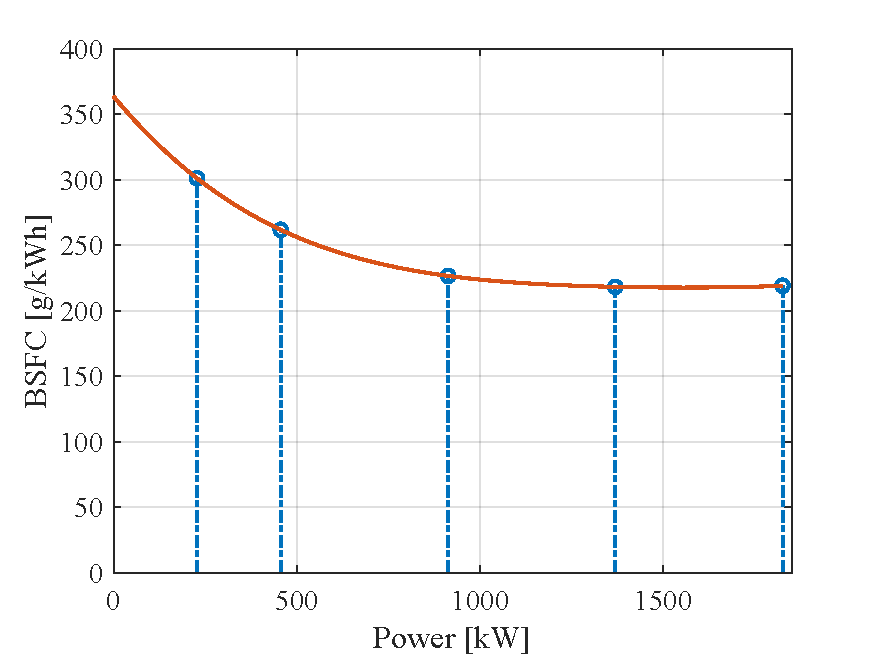
\includegraphics[scale=1]{images/chapter02/BSFC.pdf}
    \caption{Brake-specific fuel consumption (BSFC) of the \textit{CAT 3516B engine} used in tugboats.}
    \label{fig:BSFC}
\end{figure}

To analyze the operating profile, it is necessary to introduce the concept of \textbf{brake-specific fuel consumption (BSFC)}. BSFC is a measure of an engine's fuel efficiency, calculated as the amount of fuel consumed per unit of power produced over a specific time \cite{LSZ}. 

The BSFC as a function of output power is illustrated in fig. \ref{fig:BSFC} for a typical engine used in tugboats. At higher power levels, the BSFC is lower, indicating that more power is produced per unit of fuel, resulting in greater efficiency. Maximum efficiency is achieved at the engine's rated power, where it operates as intended, maintaining an optimal balance between fuel consumption and power output. Conversely, at lower power levels, the BSFC is higher, meaning that fuel consumption per unit of power is greater, thus reducing the engine efficiency.

The relative efficiency evaluates how the conventional engine is working taking as a reference the optimal efficiency at the nominal operating point as shown in eq. \ref{eq:rel_eff}. At this operating point the relative efficiency is 100$\%$ reducing its value if the engine works at lower levels of power.

\begin{align}\label{eq:rel_eff}
    \eta_\text{rel} &= \frac{\text{BSFC}_\text{nom}}{\text{BSFC}}
\end{align}

\subsection{Generated Emissions and Fuel Consumption}

To calculate emissions, the following formula relates brake power (Pb), BSFC, usage time (tu), and a carbon factor (CF):

\begin{align}
    \text{Emissions} &= \frac{\text{BSFC} \cdot {P}_{b} \cdot {t}_{u} \cdot \text{CF}}{10^{-6}} \quad \text{[t CO\textsubscript{2}]}
\end{align}

\begin{figure}[!t]
    \centering
    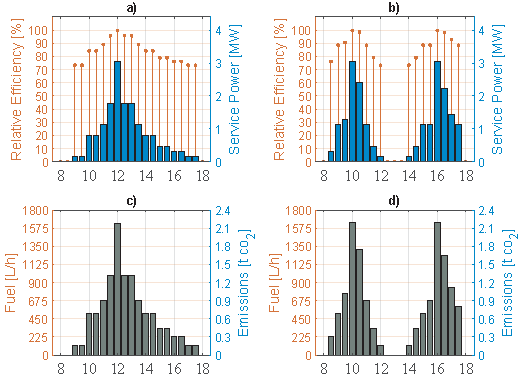
\includegraphics[width=1\linewidth]{images/chapter02/pot_30min.pdf}
    \caption{Load profile of a tugboat operating in a Chilean harbor: a) One service manoeuvre, b) Two service manoeuvres, c) Fuel consumption/emissions generated for a service maneuver, d) Fuel consumption/emissions generated for two service maneuvers.}
    \label{fig:load profile}
\end{figure}

The operational profile of a tugboat operating in a Chilean port typically includes one to two maneuvers per day during a 10-hour work shift, as illustrated in Fig. \ref{fig:load profile}.
Fig. \ref{fig:load profile}-a) shows the power delivered by the tugboat conventional propulsion system and the relative efficiency of the engines during one service maneuver while b) shows the same information for two maneuvers; c) shows the fuel consumption by the tug and the CO\textsubscript{2} emissions generated by the load of the diesel engines, corresponding to a maneuver, while d) shows the emissions generated by the load of the diesel engines for two service maneuvers.

\begin{figure}[H]
    \centering
    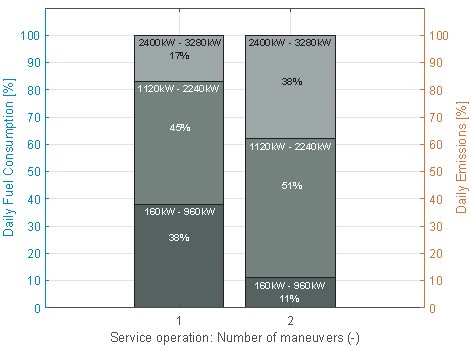
\includegraphics[width=0.9\linewidth]{images/chapter02/operations.pdf}
    \caption{Percentage of emissions per day based on power ranges.}
    \label{fig:emmis}
\end{figure}


It can be observed that as the tugboat operates close to the nominal power point of its diesel engines, its relative efficiency improves. This indicates optimal fuel consumption during those periods. Conversely, at lower operating points, the engine consumes more fuel relative to the energy produced.



Fig. \ref{fig:emmis} shows the accumulated fuel consumption and CO\textsubscript{2} emissions generated for one and two maneuvers. Each service operation is divided into three segments: the lower segments correspond to propulsion system power levels with a relative efficiency below 90\%, the middle segments correspond to relative efficiencies ranging from 90\% to 98\%, and the upper segments represent power levels with the highest relative efficiency, ranging from 98\% to 99.8\%.  At low power levels, fuel consumption can account for up to 38\% and 11\% of the total daily fuel usage, for one and two maneuvers, respectively. Resulting in high emissions due to the diesel engine operating far from its optimal efficiency point, emphasizing the variability of the load profile of this type of vessel and its impact on fuel consumption and emissions. 
 
\section{Chapter Summary}